\documentclass[preview, border=7mm]{standalone}
\usepackage{xinttools} % for the \xintFor***
\usepackage{tikz}
\usetikzlibrary{calc}


\def\biglen{20cm} % playing role of infinity (should be < .25\maxdimen)
% define the "half plane" to be clipped (#1 = half the distance between cells)
\tikzset{
  half plane/.style={ to path={
       ($(\tikztostart)!.5!(\tikztotarget)!#1!(\tikztotarget)!\biglen!90:(\tikztotarget)$)
    -- ($(\tikztostart)!.5!(\tikztotarget)!#1!(\tikztotarget)!\biglen!-90:(\tikztotarget)$)
    -- ([turn]0,2*\biglen) -- ([turn]0,2*\biglen) -- cycle}},
  half plane/.default={1pt}
}

\def\n{7} % number of random points
\def\maxxy{4} % random points are in [-\maxxy,\maxxy]x[-\maxxy,\maxxy]

\begin{document}
\begin{center}
  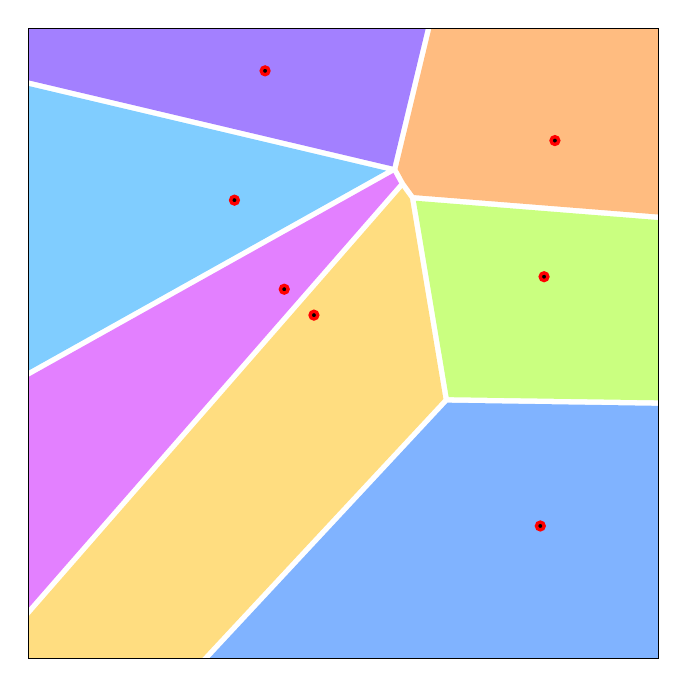
\begin{tikzpicture}
    % generate random points
    \pgfmathsetseed{14} % init random with the year Voronoi published his paper ;)
    \def\pts{}
    \xintFor* #1 in {\xintSeq {1}{\n}} \do{
      \pgfmathsetmacro{\ptx}{.9*\maxxy*rand} % random x in [-.9\maxxy,.9\maxxy]
      \pgfmathsetmacro{\pty}{.9*\maxxy*rand} % random y in [-.9\maxxy,.9\maxxy]
      \edef\pts{\pts, (\ptx,\pty)} % stock the random point
    }

    % draw the points and their cells
    \xintForpair #1#2 in \pts \do{
      \edef\pta{#1,#2}
      \begin{scope}
        \xintForpair \#3#4 in \pts \do{
          \edef\ptb{#3,#4}
          \ifx\pta\ptb\relax % check if (#1,#2) == (#3,#4) ?
            \tikzstyle{myclip}=[];
          \else
            \tikzstyle{myclip}=[clip];
          \fi;
          \path[myclip] (#3,#4) to[half plane] (#1,#2);
        }
        \clip (-\maxxy,-\maxxy) rectangle (\maxxy,\maxxy); % last clip
        \pgfmathsetmacro{\randhue}{rnd}
        \definecolor{randcolor}{hsb}{\randhue,0.5,1}
        \fill[randcolor] (#1,#2) circle (4*\biglen); % fill the cell with random color
        \fill[draw=red,very thick] (#1,#2) circle (1.4pt); % and draw the point
      \end{scope}
    }
    \pgfresetboundingbox
    \draw (-\maxxy,-\maxxy) rectangle (\maxxy,\maxxy);
  \end{tikzpicture}
\end{center}
\end{document}